\section {Implementation of UserCSP}
\label{sec:imp}

\begin{figure}[!ht]
\begin{center}
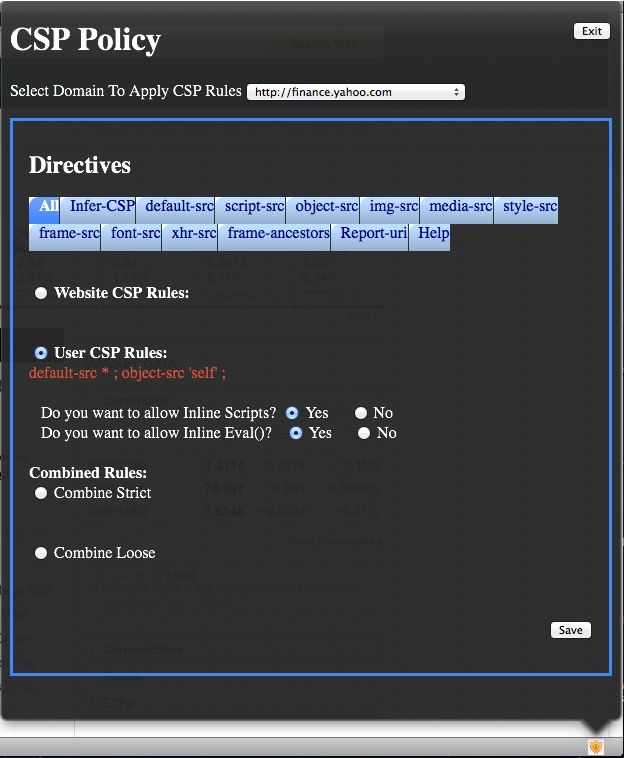
\includegraphics[width=0.7\textwidth]{UserCSP-ui}
\end{center}
\caption{UserCSP UI}
\label{fig:userCSP-ui}
\end{figure}

We implemented UserCSP \footnote[1]{UserCSP Source Code:
  https://github.com/patilkr/userCSP} in Firefox extension using the
Jetpack SDK v1.9~\cite{JetPack-SDK}. UserCSP intercepted various
events, including the {\it READY}, {\it ACTIVATE}, and {\it CLOSE} events on
tab. The READY event is used to retrieve a list of open websites in a
user's Firefox web browser. The ACTIVATE event is used to select the
currently active domain in the web browser.  The CLOSE event is used
to remove the domain name from the UI if a user closes the
tab. UserCSP uses a sqlite database to store user specified CSP rules
for websites.

The {\it http-on-examine-response} observer notification is used to
intercept the HTTP response. In the intercepted response, the domain
that initiated the request is checked against the sqlite local
database to determine whether user defined rules were set. If there
are no rules associated with the website, the response is processed
without any change.  However, if user defined CSP rules exist, the
{\tt Content- Security-Policy} header is added to the response with
the rules specified by the user. If user has opted to enforce their
own rules then UserCSP replaces the existing {\tt Content-Security-Policy} header if it is already set by the website.

Figure~\ref{fig:userCSP-ui} shows graphical user interface of UserCSP
add-on we developed as an extension to Mozilla Firefox. The userCSP
add-on UI contains drop-down list for domain selection. The domain
selection list contains the websites that the user has opened in the
browser. For example, \url{http://finance.yahoo.com/} is shown in the
Figure. In addition to this, domain selection drop-down list also
contains an entry {\tt * (Every Website)}. The {\tt * (Every Website)}
option is used to allow users to specify general rules for all
websites the users visits that do not have a website or user CSP
policy set. If a user has set a policy for website and also set a
policy for {\tt * (Every Website)}, then the user policy set for the
website takes precedence over the {\tt * (Every Website)}. If a
website has set a CSP policy in their header and the user has set a
policy for {\tt * (Every Website)}, then the policy set by the website
takes precedence over the {\tt * (Every Website)}.

Moreover, for each domain there are total 14 tabs provided to user as
shown in the Figure~\ref{fig:userCSP-ui} namely, {\tt All, Infer-CSP,
  default-src, script-src, object-src, image-src, media-src,
  style-src, frame-src, font-src, xhr-src, frame-ancestors,
  report-uri, Help}. Except for the 'All', 'Infer Policy', and 'Help'
tab, the other tabs are CSP directives used in Firefox. They are used
to allow a user to specify a CSP rule for that CSP directive. The
'All' tab is used to display the complete website defined CSP policy,
as well as complete user defined CSP policy. It also allows users to
calculate the Strictest Policy and Loosest Policy from the user
defined CSP and the website defined CSP. Moreover, it also allows user
to select a policy for a website from the four possible values -
Website CSP rules, User CSP rules, Combine Strict Rules or Combine
Loose Rules. By-default website CSP rules are selected. In addition to
this, when the User CSP rules are selected, the 'All' tab also allows
users to enable or disable inline scripts and inline evals.

\paragraph{\bf Combine Strict CSP:} If both website and user defined CSP rules for a website are available then this feature allow users to apply the strictest subset CSP policy which is calculated from the website defined CSP and the user defined CSP. For example, when you strictly combine website specified policy {\tt img-src 'self'} with user specified policy {\tt img-src '*'}, the combined policy {\tt img-src 'self'} is set.

\paragraph{\bf Combine Loose CSP:} If both website and user defined CSP rules for a website are available then this feature allow users to apply the loosest subset CSP policy which is calculated from the website defined CSP and the user defined CSP. For example, when you loosely combine website specified policy {\tt img-src 'self'} with user specified policy {\tt img-src "*"}, the combined policy {\tt img-src '*'} is set.

\tanvi{ [Kailas - unless the user has selected to apply website rules
    instead of their own rules.  Maybe add something about that]}

